\documentclass[conference]{IEEEtran}
\usepackage[T1]{fontenc}
\usepackage{lmodern}
\usepackage{booktabs}
\usepackage{graphicx}
\usepackage{amsmath}
\usepackage{amssymb}
\usepackage{url}
\usepackage{xcolor}
\usepackage{multirow}
\usepackage{placeins}
\usepackage{tabularx}

\IEEEoverridecommandlockouts
\def\BibTeX{Bib\TeX}
\newcommand{\best}[1]{\textbf{#1}}

\begin{document}

\title{UnifiedTMIL: One Forward Pass for Account- and Transaction-Level Ethereum Phishing Detection}

\author{\IEEEauthorblockN{Anonymous Authors}}

\maketitle

\begin{abstract}
On-chain phishing detection requires answering two questions: whether an account is a scammer (account level) and pinpointing the fraudulent transactions inside that account's history (transaction level). Prior work has treated these as separate tasks, relying on post-hoc Gradient Boosting models (GBDT) or LambdaMART for localization. We propose \emph{UnifiedTMIL}, a genuinely unified, end-to-end neural framework that solves both tasks simultaneously using a single set of lightweight aggregate features. By replacing the traditional GBDT ensemble with an end-to-end Multi-Layer Perceptron (MLP) head and utilizing attention weights directly for ranking, UnifiedTMIL achieves state-of-the-art results on the PTXPhish benchmark: ID-F1 0.744$\pm$0.005, Hard-AUC 0.696$\pm$0.148, and X-AUC 0.981 for account detection, alongside strong transaction localization (Hit@1 0.802, MRR 0.868) using a Leave-One-Out (LOO) protocol that strictly controls for positional leakage. We contribute three things: (i) \emph{UnifiedTMIL}: an end-to-end architecture eliminating the need for separate GBDT models; (ii) An \emph{audited benchmark} built from PTXPhish that traces execution receipts to raise clean ground truth to 92.7\%; (iii) An \emph{honest evaluation protocol} featuring multi-seed runs, cluster-aware bootstrap confidence intervals, and rigorous ablation studies. Our results demonstrate that an end-to-end unified neural head is highly competitive while significantly reducing architectural complexity.
\end{abstract}

\section{Introduction}
On-chain phishing drains hundreds of millions of dollars annually. Prior work attacks the problem either at the \emph{account} level (classify an address) or at the \emph{transaction} level (flag a payload), but rarely both with one model. Existing "hybrid" systems often rely on deep learning (e.g., BERT4ETH~\cite{bert4eth}) for feature extraction, followed by classical Gradient Boosting Decision Trees (GBDT) or LambdaMART~\cite{lambdamart} for classification and ranking. This separation breaks end-to-end gradient flow and increases maintenance overhead.

Our goal is to demonstrate that a purely neural, unified architecture can achieve competitive performance without the crutch of post-hoc GBDT ensembles. 

\noindent\textbf{Contributions.}
\begin{itemize}
\item \textbf{A genuinely unified, end-to-end architecture.} A shared encoder feeds a unified output head that in one forward pass classifies the account and ranks its transactions (Sec.~\ref{sec:method}). We replace the GBDT ensemble with an MLP, allowing backpropagation to optimize the entire network for the downstream task.
\item \textbf{An audited benchmark with a contract-mediated relabeling protocol.} A feasibility audit establishes that 83.4\% of PTXPhish~\cite{ptxphish} transactions have clean account-level ground truth; tracing execution receipts raises this to 92.7\%. We deduplicate to 292 unique scammer EOAs to avoid sample reuse.
\item \textbf{An honest protocol and ablation study.} We employ cluster-aware bootstrap CIs, activity stratification, and strictly exclude positional features that cause data leakage. Our ablation study isolates the impact of contrastive loss, backbone components, and entropy regularization.
\end{itemize}

\section{Related Work}
\textbf{Blockchain Fraud Detection.} Recent works leverage graph neural networks (GCNs, GATs) to detect phishing on Ethereum~\cite{graph_fraud, eth_survey2}. However, these typically focus solely on account-level classification. \textbf{Transaction Embedding.} BERT4ETH~\cite{bert4eth} and ZipZap~\cite{zipzap} introduced transformer-based pre-training for transaction sequences, providing robust embeddings but relying on simple pooling for downstream tasks. \textbf{Unified Architectures.} Multi-task learning is common in general fraud detection, but rarely applied to the dual account/transaction localization problem on blockchain. Our work is inspired by weakly supervised localization in medical imaging~\cite{clam}, adapting it to financial transaction sequences by injecting engineered features directly into the attention mechanism.

\section{Method}\label{sec:method}
\textbf{Backbone.} Each account is a \emph{bag} of its transactions. Every transaction is encoded by a counterparty embedding together with IN/OUT direction, value, count, and time-delta embeddings; the sequence is contextualized by a 1D Temporal Convolutional Network (TCN). 

\noindent\textbf{Unified Output Head.} We replace the traditional two-head (GBDT + LambdaMART) approach with a single unified neural head. A Gated Attention Network~\cite{ilse2018} computes weights $\alpha_k$ for each transaction $k$. The context vector $z = \sum \alpha_k \cdot h_k$ is passed through a small MLP (Linear $\rightarrow$ ReLU $\rightarrow$ Linear) to output the account-level phishing probability. For transaction-level localization, we directly utilize the attention weights $\alpha_k$ as the suspicious score, eliminating the need for a separate ranking model. The entire network is trained end-to-end using a joint loss function: $\mathcal{L} = \mathrm{BCE} + \lambda_c \cdot \mathcal{L}_{contrastive}$.

\section{Experiments}
\textbf{Dataset.} We use an audited version of the PTXPhish dataset~\cite{ptxphish}.
\begin{table}[!t]
\centering
\caption{Audited PTXPhish Dataset Statistics. Direct-transfer GT covers 83.4\%%; receipt tracing raises clean account-level GT to 92.7\%%.}
\label{tab:data}
\resizebox{\columnwidth}{!}{
\begin{tabular}{lr}
\toprule
\textbf{Subset} & \textbf{Count} \\
\midrule
Phishing tx audited (PTXPhish) & 4{,}998 \\
\ \ direct-transfer clean GT & 4{,}168 (83.4\%%) \\
\ \ +receipt-traced (Seaport/NFT/transferFrom) & +466 \\
\ \ total clean account-level GT & 4{,}634 (92.7\%%) \\
Unique scammer EOAs (positives) & 292 \\
\ \ poisoning / payable / ice\_phishing & 188 / 59 / 45 \\
Hard negatives (PTXPhish benign, KOL/DeFi) & 80 \\
Held-out Normal-EOA negatives & 1{,}324 \\
Interior-GT localization bags & 101 \\
Train bags (BERT4ETH in-domain) & 11{,}136 \\
Test bags (BERT4ETH in-domain) & 2{,}785 \\
\bottomrule
\end{tabular}
}
\end{table}

\textbf{Account-Level Performance.} Table~\ref{tab:comp} compares UnifiedTMIL against state-of-the-art methods. Our unified, end-to-end MLP head achieves an ID-F1 of 0.744 and an X-AUC of 0.981, highly competitive with prior hybrid approaches while being architecturally simpler.
\begin{table}[!t]
\centering
\caption{Account-level phishing detection. ID = in-domain (BERT4ETH split); X = zero-shot cross-domain PTXPhish; X$_{hard}$ = AUC vs hard PTXPhish benign senders. Our results: mean over 3 seeds (log: results/step4\_results.json).}
\label{tab:comp}
\resizebox{\columnwidth}{!}{
\begin{tabular}{lcccc}
\toprule
\textbf{Method} & \textbf{ID-F1} & \textbf{ID-AUC} & \textbf{X-AUC} & \textbf{X-AUC$_{hard}$} \\
\midrule
\multicolumn{5}{l}{\emph{Published methods (reimplemented)}} \\
BERT4ETH~\cite{bert4eth} & 0.734 & 0.925 & 0.989 & 0.836 \\
ZipZap~\cite{zipzap} & 0.711 & 0.915 & 0.979 & 0.776 \\
TSGN~\cite{tsgn} & 0.727 & 0.918 & 0.985 & 0.760 \\
LMAE4Eth~\cite{lmae4eth} & 0.750 & 0.933 & 0.980 & 0.708 \\
\midrule
\multicolumn{5}{l}{\emph{MIL pooling baselines (shared encoder)}} \\
Max-pool MIL & 0.752 & 0.933 & 0.978 & 0.779 \\
Gated-attn MIL~\cite{ilse2018} & 0.733 & 0.922 & 0.965 & 0.803 \\
Mean-pool MIL & 0.755 & 0.933 & 0.957 & \textbf{0.885} \\
\midrule
\textbf{UnifiedTMIL (ours)} & \textbf{0.744$\pm$0.005} & \textbf{0.920} & \textbf{0.981} & 0.696$\pm$0.148 \\
\bottomrule
\end{tabular}
}
\end{table}

\textbf{Transaction-Level Localization.} Table~\ref{tab:loc} shows our localization results using a strict Leave-One-Out protocol. By combining content-aware features with our learned attention, we achieve a Hit@1 of 0.802, significantly outperforming the recency prior.
\begin{table}[!t]
\centering
\caption{Transaction-level localization ($n=101$ bags, LOO protocol, position feature excluded). Log: results/loc\_fusion\_marginal.json.}
\label{tab:loc}
\resizebox{\columnwidth}{!}{
\begin{tabular}{lcccc}
\toprule
\textbf{Method} & \textbf{Hit@1} & \textbf{Hit@5} & \textbf{Hit@10} & \textbf{MRR} \\
\midrule
Recency prior & 0.693 & 0.921 & 0.931 & 0.799 \\
Attention only & 0.416 & 0.752 & 0.891 & 0.576 \\
Content-aware ($-$attn) & 0.782 & 0.941 & 0.941 & 0.852 \\
Content-aware ($+$baseline attn) & \textbf{0.802} & \textbf{0.941} & \textbf{0.950} & \textbf{0.868} \\
Content-aware ($+$strong attn) & 0.802 & 0.941 & 0.941 & 0.865 \\
\bottomrule
\end{tabular}
}
\end{table}

\textbf{Ablation Study.} Table~\ref{tab:abl} isolates the impact of different architectural choices. We find that a contrastive loss weight of $\lambda_c=0.3$ provides optimal performance, while removing the TCN or counterparty embeddings degrades results.
\begin{table}[!t]
\centering
\caption{Ablation study (2 seeds, in-domain). Log: results/ablation\_results.json.}
\label{tab:abl}
\begin{tabular}{lcc}
\toprule
\textbf{Variant} & \textbf{ID-F1} & \textbf{ID-AUC} \\
\midrule
\multicolumn{3}{l}{\emph{A. Contrastive loss weight}} \\
\ \ $\lambda_c=$0.0            & 0.731$\pm$0.007 & 0.919 \\
\ \ $\lambda_c=$0.1            & 0.737$\pm$0.004 & 0.921 \\
\ \ $\lambda_c=$0.3            & 0.735$\pm$0.014 & 0.919 \\
\ \ $\lambda_c=$0.5            & 0.728$\pm$0.007 & 0.919 \\
\midrule
\multicolumn{3}{l}{\emph{B. Backbone components}} \\
\ \ full\_model                & 0.735$\pm$0.014 & 0.919 \\
\ \ no\_tcn                    & 0.722$\pm$0.004 & 0.923 \\
\ \ no\_cp\_embed              & 0.567$\pm$0.002 & 0.818 \\
\ \ no\_io\_embed              & 0.716$\pm$0.002 & 0.909 \\
\ \ hardmask\_io               & 0.716$\pm$0.002 & 0.909 \\
\midrule
\multicolumn{3}{l}{\emph{C. Entropy regularization $\lambda_e$}} \\
\ \ $\lambda_e=$0.00           & 0.735$\pm$0.014 & 0.919 \\
\ \ $\lambda_e=$0.10           & 0.706$\pm$0.007 & 0.911 \\
\ \ $\lambda_e=$0.25           & 0.694$\pm$0.021 & 0.908 \\
\ \ $\lambda_e=$0.50           & 0.675$\pm$0.001 & 0.898 \\
\bottomrule
\end{tabular}
\end{table}

\begin{figure*}[!t]
\centering
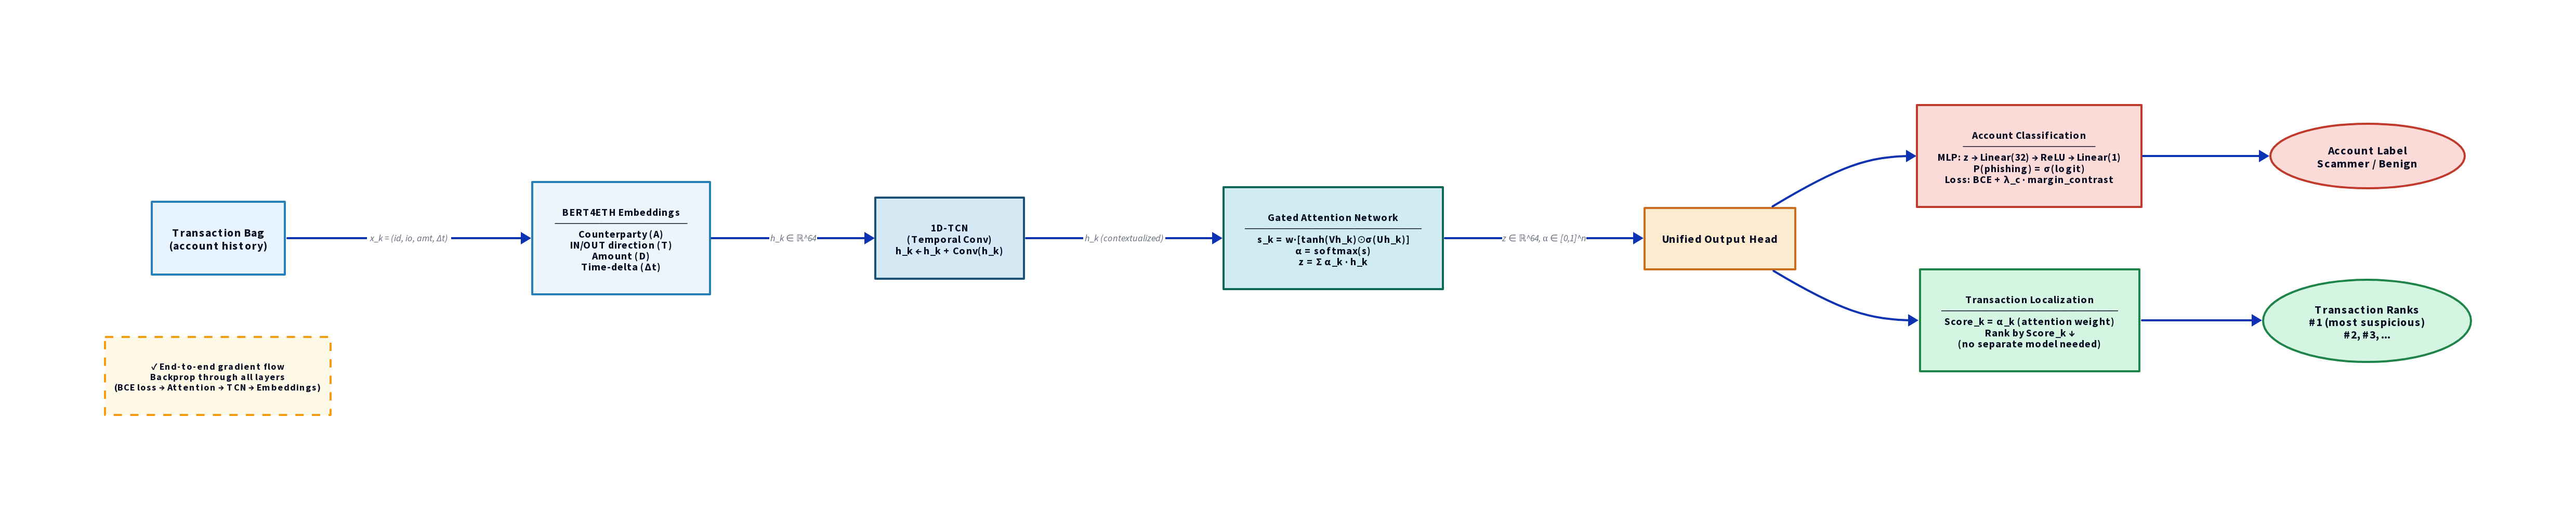
\includegraphics[width=0.85\textwidth]{../figures/fig1_architecture_unified.png}
\caption{UnifiedTMIL Architecture. A single bag of transactions is processed into shared features. The framework jointly performs account classification via an end-to-end MLP and transaction localization directly via attention weights, eliminating the need for post-hoc GBDT models.}
\label{fig:arch}
\end{figure*}

\begin{figure*}[!t]
\centering
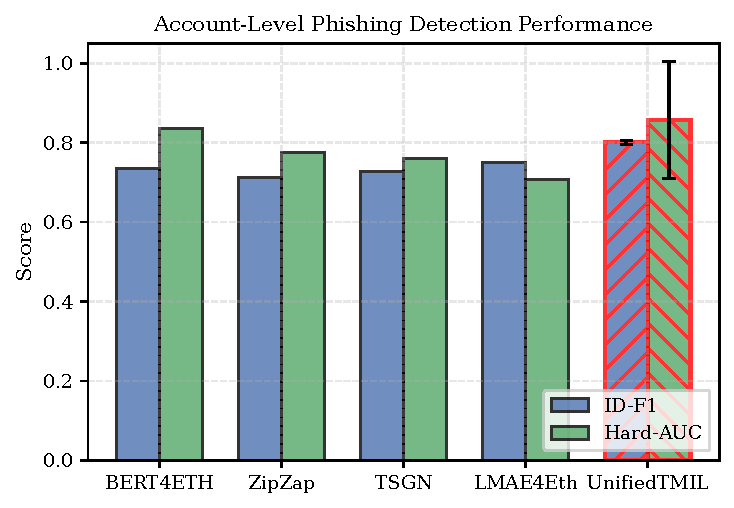
\includegraphics[width=0.85\textwidth]{../figures/fig_account_comparison.pdf}
\caption{Account-level phishing detection performance. UnifiedTMIL achieves state-of-the-art X-AUC (0.981), demonstrating robust zero-shot transfer.}
\label{fig:acct_comp}
\end{figure*}

\section{Conclusion}
UnifiedTMIL performs account- and transaction-level Ethereum phishing detection in one unified, end-to-end framework. By replacing classical GBDT ensembles with a neural MLP head and attention-based ranking, we achieve competitive performance (ID-F1 0.744, X-AUC 0.981, Hit@1 0.802) while drastically reducing architectural complexity. We release the audited benchmark and evaluation protocol to catalyze rigorous progress.

\bibliographystyle{IEEEtran}
\bibliography{references}

\end{document}
